% !TEX program = lualatex
\documentclass[border=6pt]{standalone}
% ---------------------------------------------------------------------------
% tikzpreamble.tex -- shared by main.tex and by every standalone in tikz/
% ---------------------------------------------------------------------------
\usepackage{amsmath}
\usepackage{amssymb}
\usepackage{tikz}
\usepackage{circuitikz}
\usetikzlibrary{arrows.meta,calc,positioning,decorations.pathmorphing,decorations.pathreplacing,
                decorations.markings,patterns,angles,quotes,fit,
                shapes.geometric,shapes.misc,backgrounds,intersections}

\ctikzset{bipoles/length=0.85cm}
\ctikzset{resistors/scale=0.85}
\ctikzset{capacitors/scale=0.9}

\tikzset{
  wire/.style      = {line width=0.7pt},
  dashedwire/.style= {line width=0.7pt, densely dashed},
  term/.style      = {circle, draw, line width=0.6pt, fill=white,
                      inner sep=0pt, minimum size=4.5pt},
  node dot/.style  = {circle, fill=black, inner sep=0pt, minimum size=4pt},
  boxlabel/.style  = {font=\sffamily\small},
  annot/.style     = {font=\small, align=left},
  phasor/.style    = {-{Stealth[length=3.2mm,width=2.2mm]}, line width=1.1pt},
  thinphasor/.style= {-{Stealth[length=2.6mm,width=1.8mm]}, line width=0.7pt},
  axis line/.style = {-{Stealth[length=2.6mm,width=1.8mm]}, line width=0.6pt},
  guide/.style     = {densely dashed, line width=0.4pt, gray},
}
\usepackage{siunitx}

\begin{document}
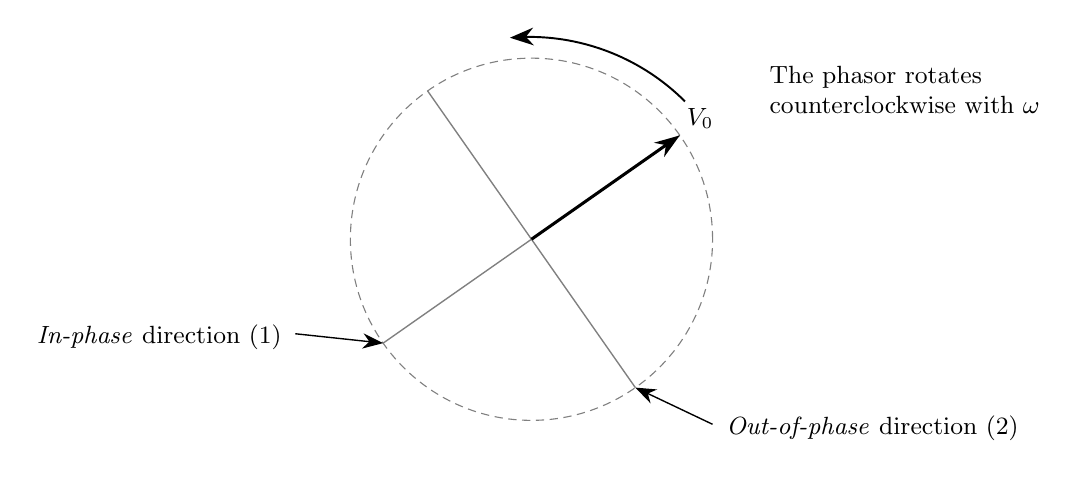
\begin{tikzpicture}[every node/.style={font=\small}]
  \def\R{2.3}
  \draw[densely dashed,gray] (0,0) circle (\R);
  % the two reference directions
  \draw[line width=0.5pt,gray] (215:\R) -- (35:\R);
  \draw[line width=0.5pt,gray] (305:\R) -- (125:\R);

  \draw[phasor] (0,0) -- (35:\R) node[anchor=south west,inner sep=2pt] {$V_0$};

  \draw[-{Stealth[length=3mm]},line width=0.7pt]
       (1.95,1.75) arc[start angle=45,end angle=95,radius=2.8];
  \node[annot,anchor=west] at (2.9,1.9)
       {The phasor rotates\\ counterclockwise with $\omega$};

  \draw[-{Stealth[length=2.6mm]},line width=0.5pt] (-3.0,-1.2) -- (215:\R);
  \node[annot,anchor=east] at (-3.05,-1.25) {\textit{In-phase} direction (1)};

  \draw[-{Stealth[length=2.6mm]},line width=0.5pt] (2.3,-2.35) -- (305:\R);
  \node[annot,anchor=west] at (2.35,-2.4) {\textit{Out-of-phase} direction (2)};
\end{tikzpicture}
\end{document}
